\section{Kiến trúc hệ thống thử nghiệm}

Hạ tầng gồm bốn VPC trong \texttt{us-east-1a}. Mỗi VPC có một subnet và một
EC2. Các private IP được gán cố định trong Terraform, trình bày tại Bảng
\ref{tab:endpoints}.

\begin{table}[H]
\centering
\caption{Endpoint được giữ nguyên giữa hai mode}
\label{tab:endpoints}
\begin{tabular}{llll}
\toprule
\textbf{Nút} & \textbf{VPC CIDR} & \textbf{Subnet CIDR} & \textbf{Private IP} \\
\midrule
A & 10.10.0.0/16 & 10.10.10.0/24 & 10.10.10.212 \\
B & 10.20.0.0/16 & 10.20.10.0/24 & 10.20.10.155 \\
C & 10.30.0.0/16 & 10.30.10.0/24 & 10.30.10.212 \\
D & 10.40.0.0/16 & 10.40.10.0/24 & 10.40.10.155 \\
\bottomrule
\end{tabular}
\end{table}

Bốn máy dùng \texttt{c6i.large}, cùng AMI
\texttt{ami-0d27e0fb3bac4d724}, root volume gp3 8 GiB và IMDSv2 bắt buộc.
Elastic IP phục vụ quản trị; traffic benchmark dùng private IP nên EIP và
Internet Gateway không nằm trên đường đo.

\section{Kiến trúc VPC Peering}

Mode Peering tạo full mesh sáu connection. Mỗi route table có ba route đến ba
CIDR còn lại; target của mỗi route là peering connection tương ứng.

\begin{figure}[H]
\centering
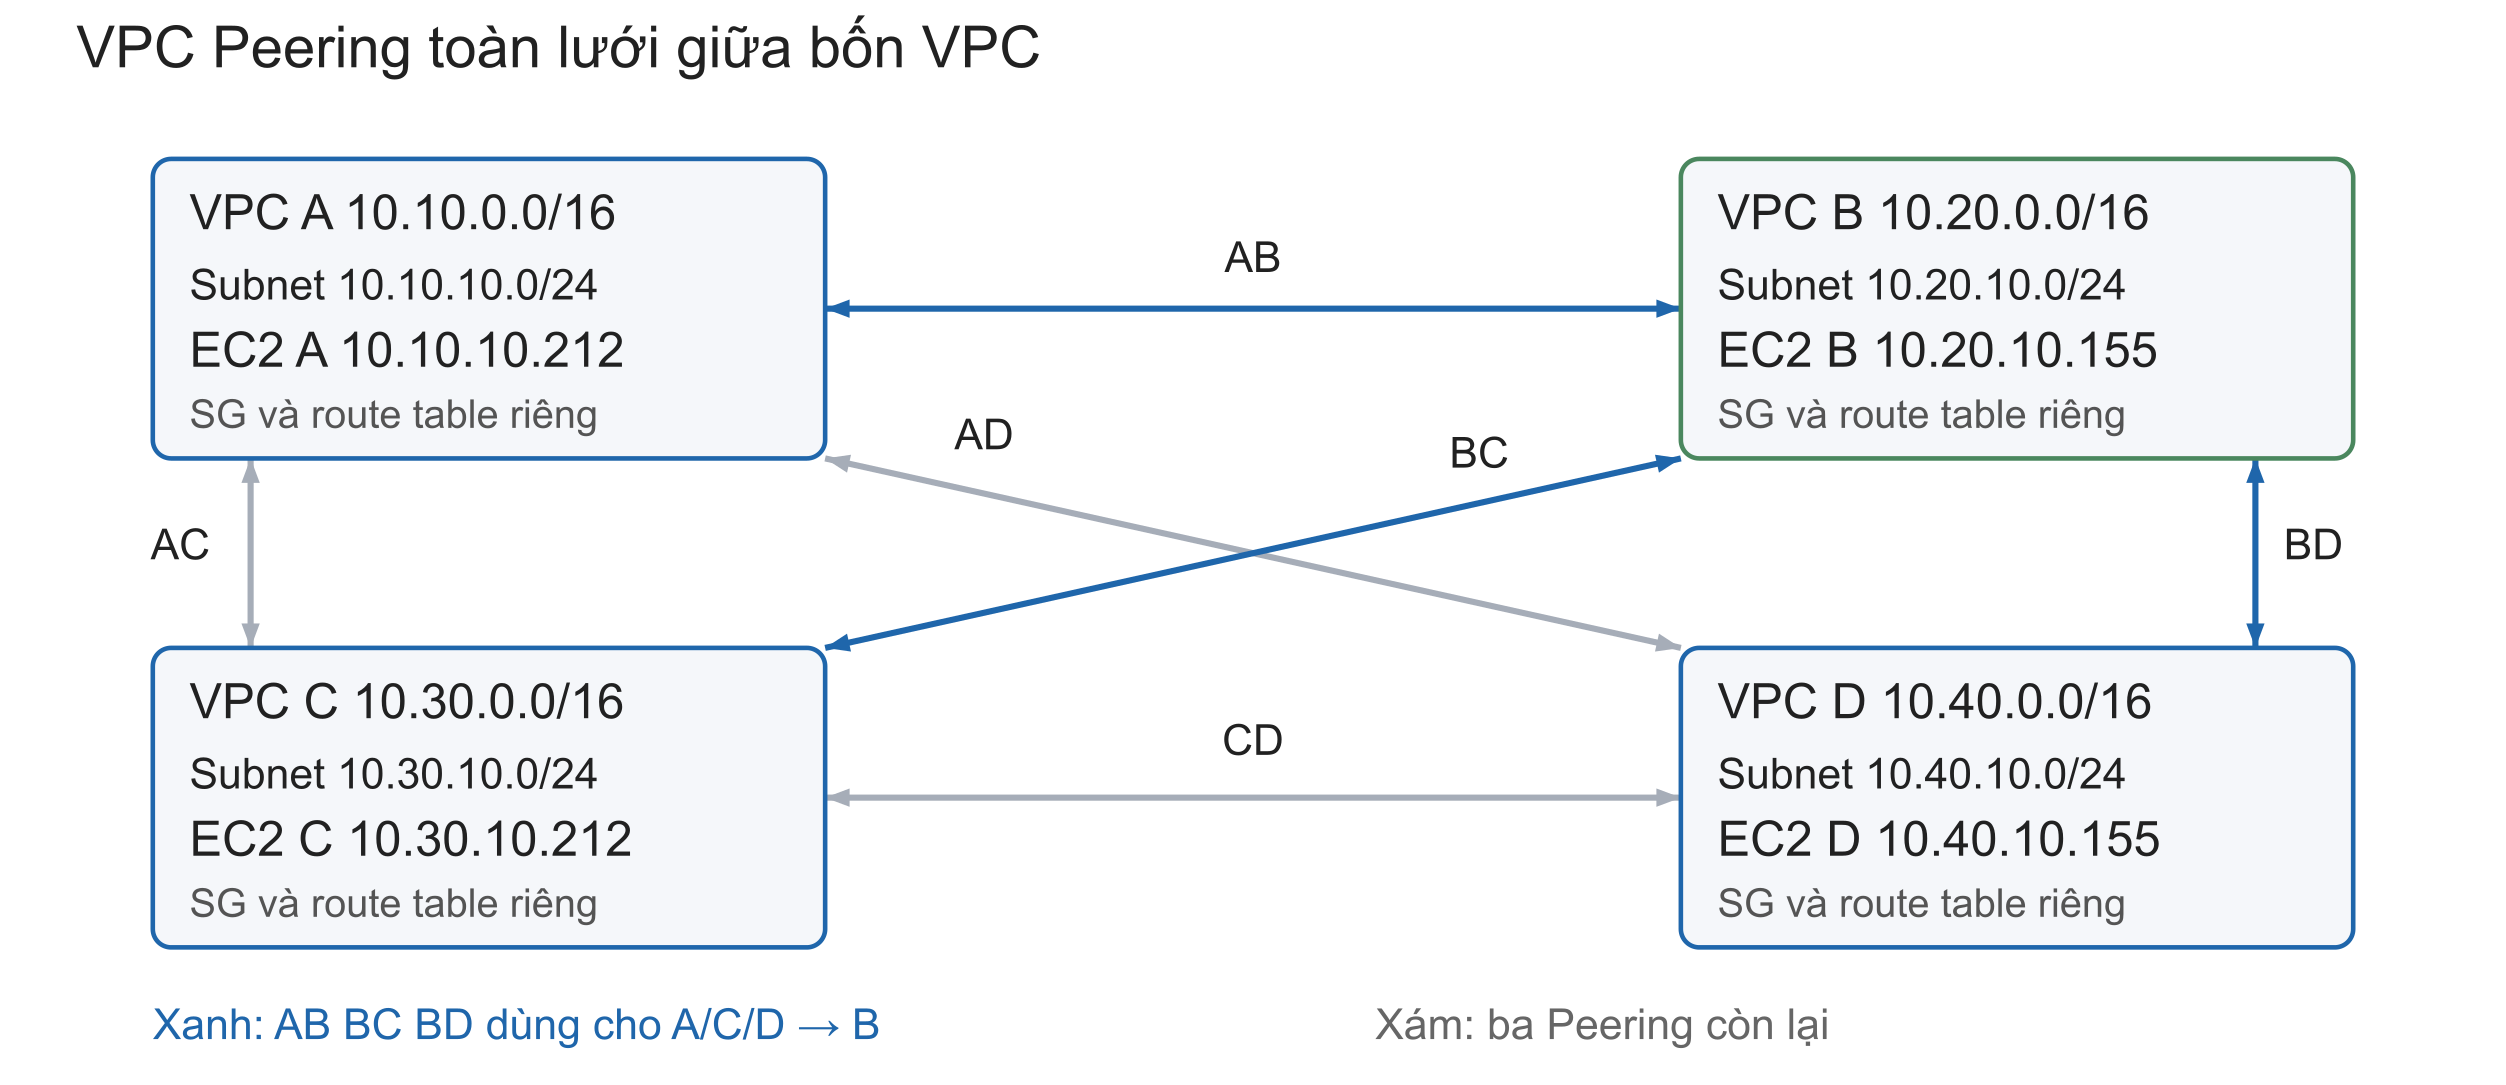
\includegraphics[width=0.92\textwidth]{img/chapter3/peering-architecture.png}
\caption{Kiến trúc thử nghiệm sử dụng VPC Peering}
\label{fig:peering-architecture}
\end{figure}

Hình \ref{fig:peering-architecture} cho thấy endpoint và địa chỉ không thay
đổi. Full mesh cung cấp đường trực tiếp cho AB, AC, AD, BC, BD và CD; không
dựa vào một VPC trung gian.

\section{Kiến trúc Transit Gateway}

Mode TGW giữ nguyên VPC, subnet và EC2 nhưng đổi target của 12 route liên VPC
sang một TGW. Mỗi VPC có một attachment tới hub.

\begin{figure}[H]
\centering
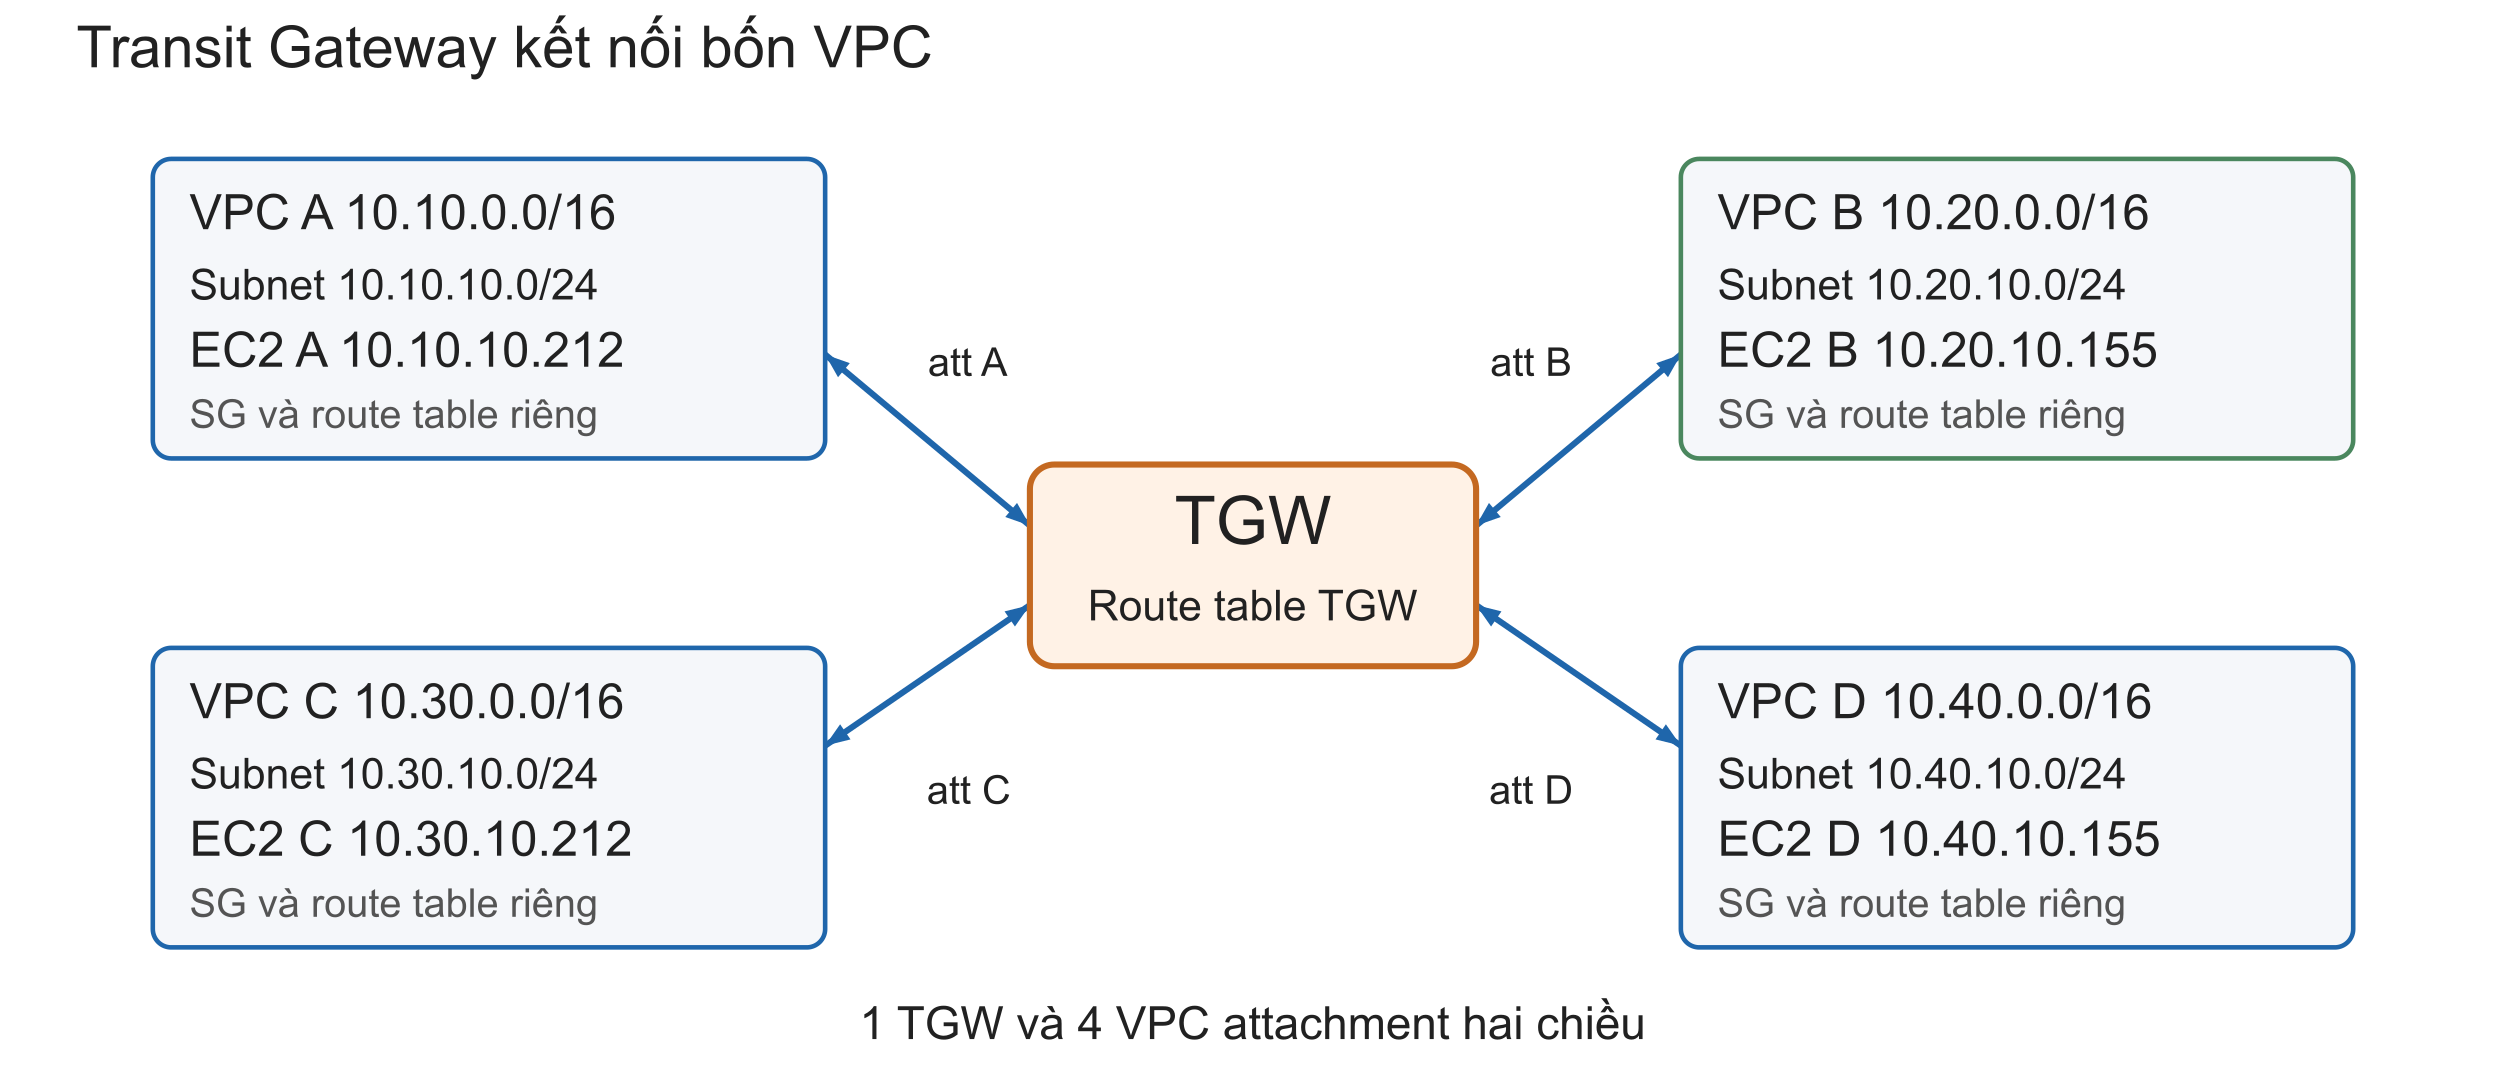
\includegraphics[width=0.92\textwidth]{img/chapter3/tgw-architecture.png}
\caption{Kiến trúc thử nghiệm sử dụng AWS Transit Gateway}
\label{fig:tgw-architecture}
\end{figure}

Hình \ref{fig:tgw-architecture} biểu diễn topology hub-and-spoke. Traffic A
tới B đi từ route table A tới TGW, qua attachment của B rồi tới EC2 B; chiều
về cần route đối ứng.

\section{Điều khiển đường đi bằng Terraform}

Hai biến quyết định mode:

\begin{itemize}
  \item \texttt{enable\_transit\_gateway}: tạo TGW và bốn attachment;
  \item \texttt{routing\_mode}: nhận \texttt{peering} hoặc \texttt{tgw} và
        chọn target cho toàn bộ 12 route liên VPC.
\end{itemize}

\begin{center}
\texttt{enable\_transit\_gateway} + \texttt{routing\_mode}
$\rightarrow$ 12 route liên VPC
$\rightarrow$ Peering target hoặc TGW target.
\end{center}

Cơ chế này quan trọng cho tính công bằng: phép đo không tạo một tập EC2 mới
cho TGW. Terraform \texttt{No changes} chỉ chứng minh desired state khớp state
đã biết; nó không tự chứng minh packet đang đi đúng đường. Vì vậy quy trình còn
lưu route snapshot và chạy connectivity check sau khi đổi mode.

\section{Đường quản trị và đường đo}

\begin{figure}[H]
\centering
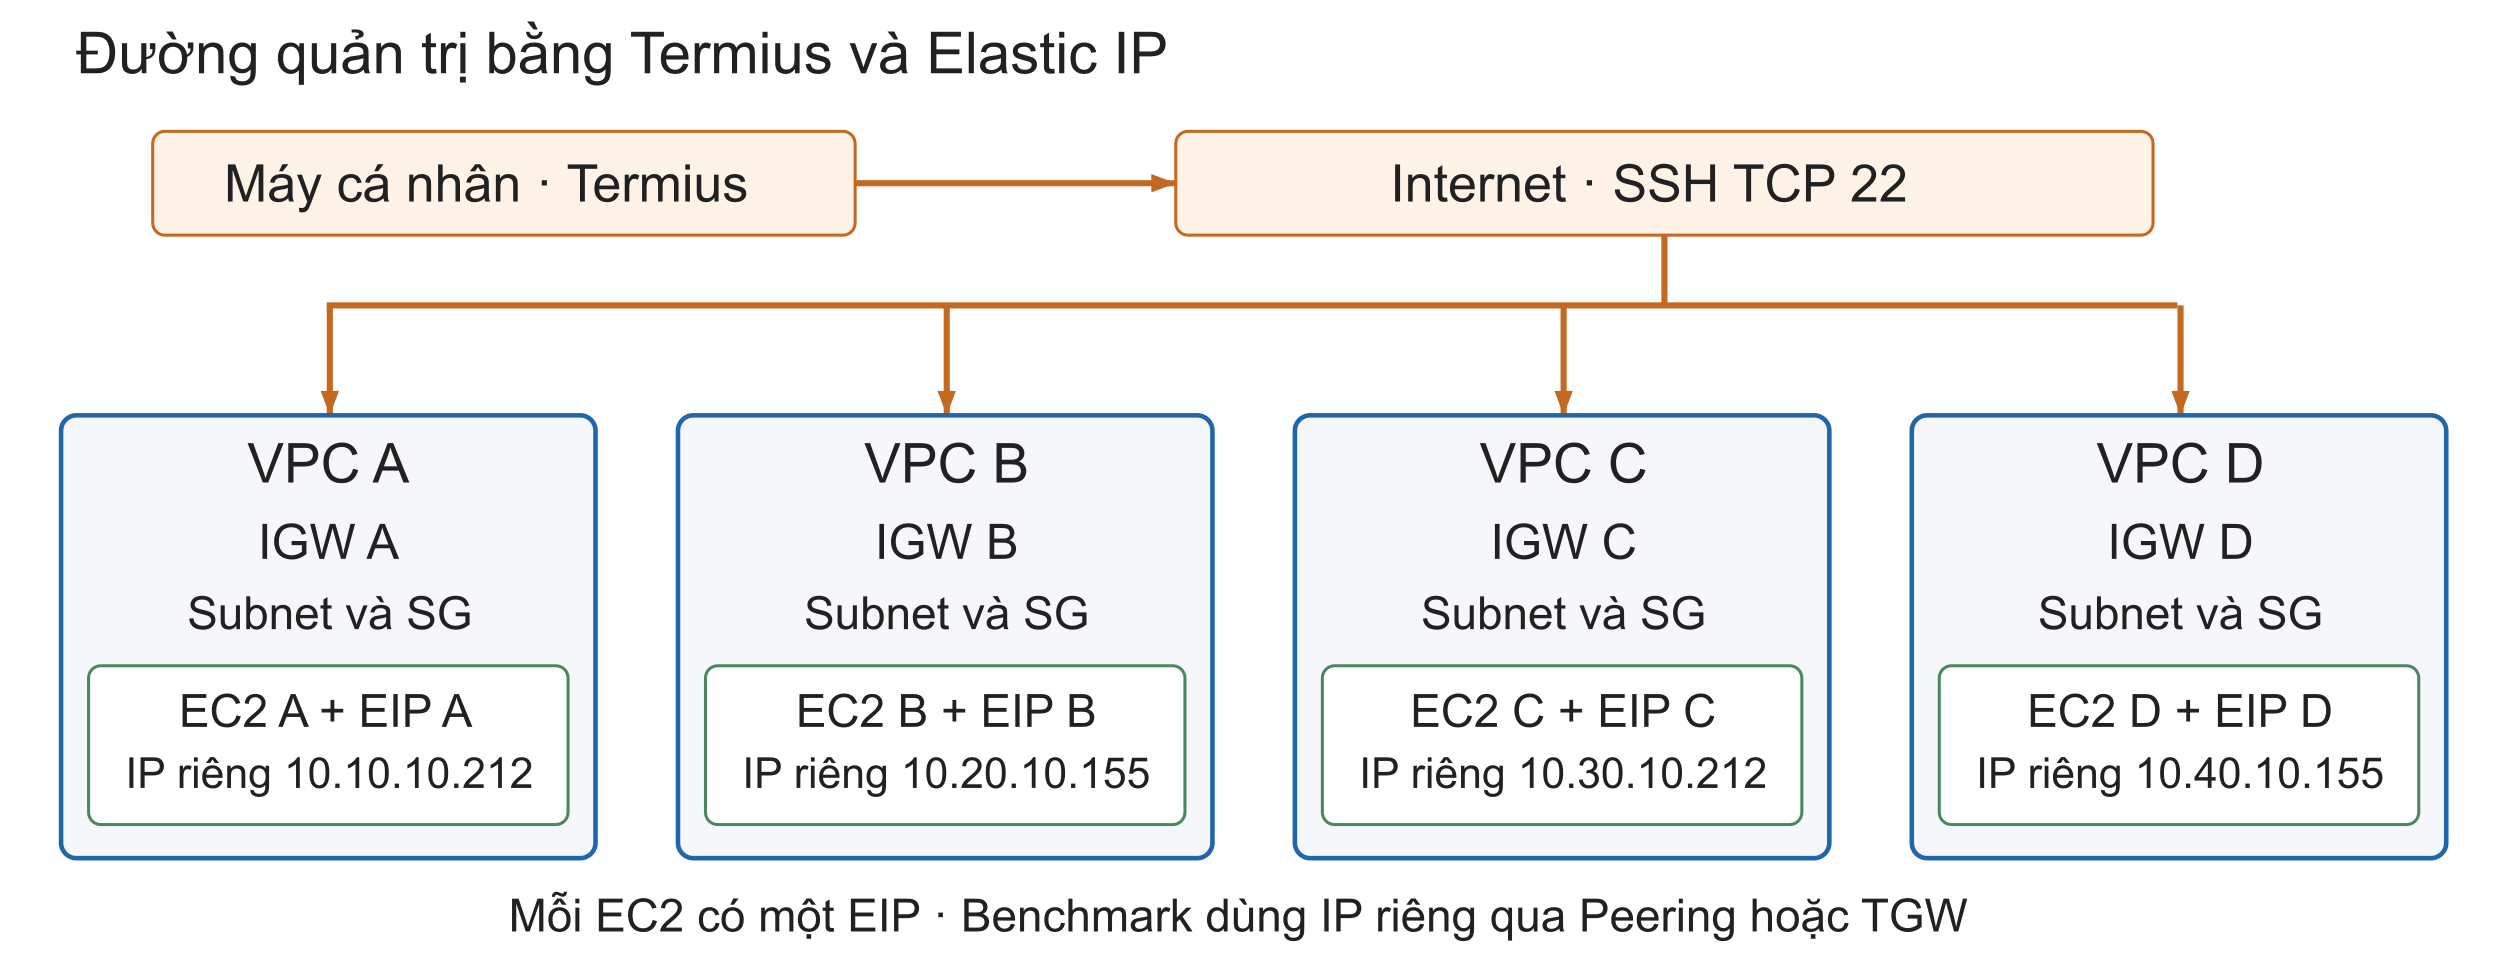
\includegraphics[width=0.92\textwidth]{img/chapter3/management-path.png}
\caption{Phân biệt Elastic IP quản trị và private IP dùng cho benchmark}
\label{fig:management-path}
\end{figure}

Elastic IP, Internet Gateway và SSH/SSM phục vụ quản trị instance. Traffic
benchmark dùng private IP và route liên VPC. Vì vậy EIP không nằm trên đường
dữ liệu được so sánh; Hình \ref{fig:management-path} chỉ mô tả control path
giúp chuẩn bị và thu thập kết quả.

\section{Điều kiện benchmark mạng}

\begin{table}[H]
\centering
\caption{Điều kiện của sáu bộ dữ liệu chính}
\label{tab:benchmark-conditions}
\begin{tabularx}{\textwidth}{p{0.28\textwidth}X}
\toprule
\textbf{Thuộc tính} & \textbf{Giá trị đã lưu} \\
\midrule
Region/AZ & \texttt{us-east-1}/\texttt{us-east-1a} \\
Instance & Bốn EC2 \texttt{c6i.large} \\
Đường dữ liệu & Private IPv4 \\
MTU & 1500 byte \\
iperf3 & 3.19.1; TCP cubic \\
TCP single-flow & Một stream, omit 5 s, đo 30 s, cổng 5201 \\
TCP fan-in & Một stream mỗi source, omit 5 s, đo 30 s, cổng 5201--5203 \\
RTT idle & 100 ICMP echo, payload 56 byte, interval 0,2 s \\
Số lượt & Năm lượt cho mỗi bài và mỗi mode \\
\bottomrule
\end{tabularx}
\end{table}

Metadata ghi NTP đồng bộ trong các phiên fan-in. Hai mode được đo nối tiếp,
không randomize hoặc counterbalance đầy đủ; đây là hạn chế phương pháp chứ
không phải chi tiết có thể bỏ qua.

\section{Công cụ đo và kiểm chứng}

\begin{itemize}
  \item \texttt{ping}: RTT, số request gửi/nhận và loss quan sát.
  \item \texttt{iperf3}: byte nhận, thời lượng, receiver bitrate,
        retransmission và JSON theo interval \cite{iperf3-docs}.
  \item \texttt{mpstat}: lấy \%idle của dòng \texttt{all}; CPU busy được tính
        bằng $100-\%idle$.
  \item \texttt{ethtool -S}: chụp ENA counter trước/sau.
  \item Terraform: tạo topology và chuyển route có kiểm soát
        \cite{terraform-aws-provider}.
  \item Python: kiểm tra checksum, parse raw data, tính metric và đối chiếu
        giữa JSON, Markdown và figures.
\end{itemize}

\section{Workload ứng dụng và thiết kế slots}

Để kiểm tra liệu network latency có phải yếu tố quyết định chất lượng dịch vụ,
nhóm triển khai một workload HTTP nhỏ trên cùng endpoint. A tạo request theo
lịch đến gateway B. B gọi C và D song song; mỗi worker thực hiện I/O mô phỏng
10 ms và trả payload JSON 4.096 byte. Hai worker có cùng giới hạn slots, lần
lượt 8 và 16. Mỗi điều kiện dùng rate 600 hoặc 800 request/s, deadline 50 ms,
timeout 2 s, warm-up 5 s, đo 15 s và drain 15 s. Mỗi block có đủ bốn điều kiện
Peering/TGW $\times$ 8/16 slots tại một mức tải; server mới được tạo cho từng
điều kiện để tránh carry-over.

\begin{table}[H]
\centering
\caption{Thiết kế workload ứng dụng}
\label{tab:application-conditions}
\begin{tabularx}{\textwidth}{p{0.26\textwidth}XX}
\toprule
\textbf{Thuộc tính} & \textbf{Giá trị} & \textbf{Ý nghĩa} \\
\midrule
Request rate & 600/800 request/s & 600 là tải dưới danh nghĩa; 800 là tải sát 8 slots \\
Worker slots & 8/16 mỗi worker & Giới hạn đồng thời của ứng dụng, không phải vCPU \\
Service/I/O & 10 ms, 4.096 byte & Workload mô phỏng có kiểm soát \\
Deadline/timeout & 50 ms/2 s & Tách đúng hạn khỏi hoàn thành muộn \\
Chỉ số & P95, SLI, queue/service time & Đo tail latency và cơ chế chờ \\
\bottomrule
\end{tabularx}
\end{table}

Một request A gọi C và D song song nên 800 request/s tạo khoảng 800 lời gọi/s
trên mỗi worker, tức 1.600 lời gọi/s khi cộng hai worker. Bảng này không gán
queue ở B cho AWS TGW; B là gateway ứng dụng.

\section{Quan sát CPU và ENA}

\texttt{mpstat} lấy mẫu CPU trong cửa sổ đo. CPU busy được tính từ dòng
\texttt{all} theo $100-\%idle$; đây là mức bận toàn máy, không phải CPU riêng
của iperf3. Lệnh \texttt{ethtool} với option \texttt{-S} trên interface
\texttt{ens5} chụp trước/sau năm counter:

\begin{itemize}
  \item \path{bw_in_allowance_exceeded} và \path{bw_out_allowance_exceeded};
  \item \path{pps_allowance_exceeded};
  \item \path{conntrack_allowance_exceeded};
  \item \path{linklocal_allowance_exceeded}.
\end{itemize}

\section{Experiment 1: RTT idle}

A gửi 100 ICMP echo tới B qua private IP. Mỗi lượt lưu raw output và summary
gồm min/avg/max/mdev. Metric so sánh là mean của năm giá trị RTT avg. Payload
56 byte và interval 0,2 s được giữ giống nhau giữa hai mode.

\section{Experiment 2: TCP single-flow}

A chạy một TCP stream tới listener B:5201. Command cốt lõi trong script là:

\begin{lstlisting}[language=bash,caption={Lệnh TCP single-flow cốt lõi},label={lst:tcp-single}]
iperf3 -c 10.20.10.155 -p 5201 -P 1 -O 5 -t 30 -i 1 -J \
  --get-server-output > "$run_file"
\end{lstlisting}

Goodput lấy từ phía nhận, không lấy bitrate phía gửi. CPU và ENA được thu ở
cả endpoint theo phạm vi mà artifact cho phép.

\section{Experiment 3: TCP fan-in}

A, C và D lần lượt gửi tới B trên cổng 5201, 5202 và 5203. Ba listener độc
lập giúp server nhận đồng thời và từng source có JSON riêng. Mỗi lượt được lên
lịch cách nhau 45 giây; thời gian bắt đầu wrapper giữa source lệch khoảng
0,78--0,82 giây trong phiên TGW. Vì cửa sổ nội bộ không trùng tuyệt đối, tổng
ba mean được gọi là tổng xấp xỉ.

\section{Quy trình chuyển Peering và TGW}

\begin{enumerate}
  \item Áp dụng mode định tuyến bằng Terraform.
  \item Kiểm tra 12 route liên VPC và target hai chiều.
  \item Chạy connectivity check giữa endpoint và các cổng đo.
  \item Chuẩn bị EC2: MTU, NTP, listener, công cụ và tiến trình cũ.
  \item Chạy benchmark với tham số cố định.
  \item Thu raw output, CPU, ENA, timestamps và metadata.
  \item Sao lưu artifact và manifest/checksum.
  \item Chạy script verify và build báo cáo kết quả.
\end{enumerate}

\section{Experiment 4: HTTP deadline và hàng đợi}

Loader A gửi request duy nhất có request ID. Gateway B truyền context ID tới C
và D, chờ cả hai worker rồi trả response. Mỗi request lưu timestamp scheduled,
entry, service start, service end và exit. Từ các timestamp này, script tính
đúng hạn, P95 hoàn thành, thời gian chờ và thời gian phục vụ. Hàng đợi được
kiểm tra lại bằng sample-path Little trên cùng cohort.

\section{OpenTelemetry và Grafana}

Collector nhận OTLP từ workload demo và chuyển trace sang Tempo; Grafana hiển
thị bảng study và waterfall. Trace được gắn nhãn smoke/historical, gồm 12 trace
và 120 span đã lưu. Pipeline chứng minh khả năng quan sát queue/service, nhưng
không được dùng để thay thế kết quả 800 request/s vì full tracing tắt trong
primary benchmark.

\section{Kết quả chính từ đợt đo xác nhận mới}

Phần này là trọng tâm thực nghiệm của báo cáo. Khác với các phiên baseline
ban đầu, đợt mới giữ nguyên cohort EC2, lưu route snapshot, đảo thứ tự mode
giữa các block và phân tích trực tiếp raw artifact. Dữ liệu gồm năm block RTT
và ba block ứng dụng, không trộn với dữ liệu pilot.

\subsection{RTT cùng cohort: 5 block và 3.000 probe}

Mỗi block đo ba lượt cho từng mode, mỗi lượt 100 ICMP echo. Toàn bộ
3.000/3.000 probe nhận được phản hồi. Hiệu ứng ghép cặp của block $j$ là

\begin{equation}
\Delta_j=\overline{RTT}_{\mathrm{TGW},j}
-\overline{RTT}_{\mathrm{Peering},j}.
\end{equation}

\begin{figure}[H]
\centering
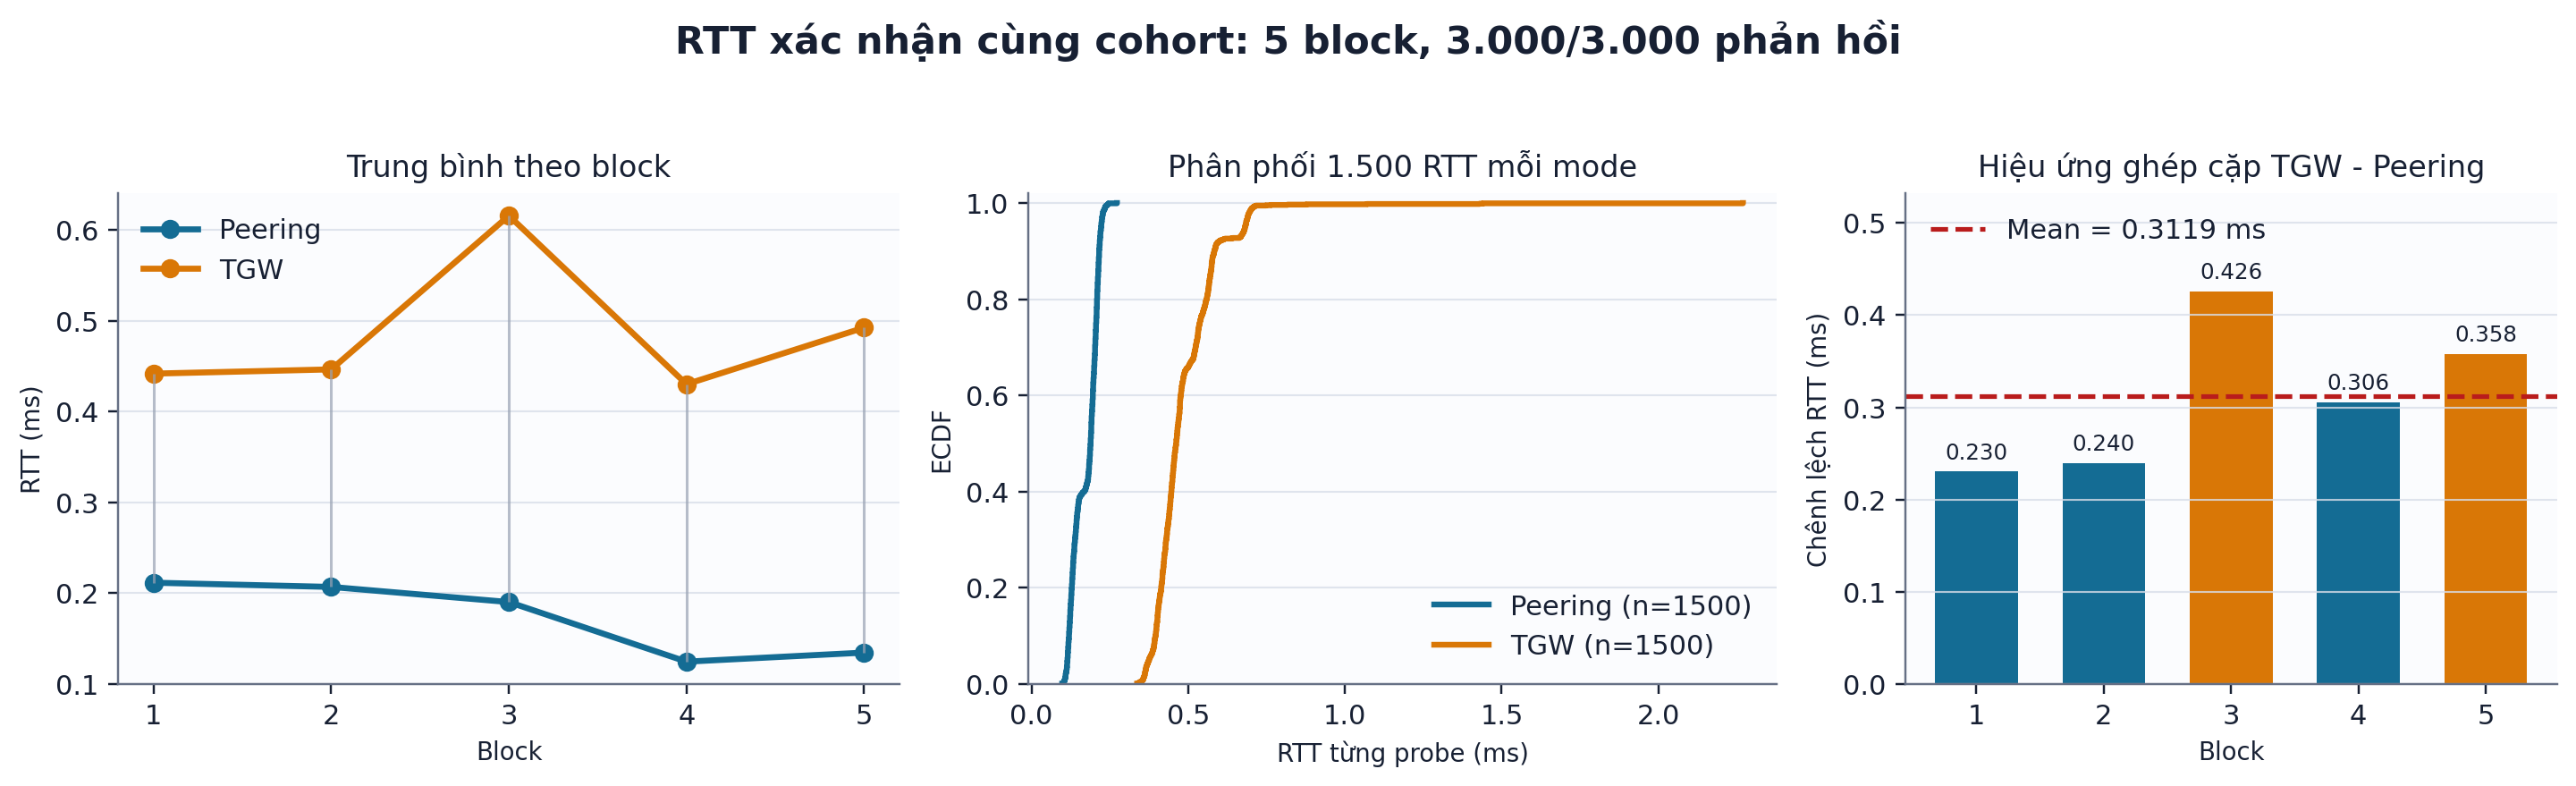
\includegraphics[width=\textwidth]{img/chapter3/primary/rtt-confirmation-dashboard.png}
\caption{Kết quả RTT mới: trung bình block, ECDF của 3.000 probe và hiệu ứng ghép cặp}
\label{fig:rtt-primary}
\end{figure}

\begin{table}[H]
\centering
\caption{RTT trung bình trong năm block xác nhận}
\label{tab:rtt-confirmation}
\begin{tabular}{crrr}
\toprule
\textbf{Block} & \textbf{Peering (ms)} & \textbf{TGW (ms)} & \textbf{$\Delta_j$ (ms)} \\
\midrule
1 & 0,2113 & 0,4417 & 0,2303 \\
2 & 0,2067 & 0,4463 & 0,2397 \\
3 & 0,1900 & 0,6157 & 0,4257 \\
4 & 0,1243 & 0,4300 & 0,3057 \\
5 & 0,1343 & 0,4923 & 0,3580 \\
\midrule
Trung bình & 0,1733 & 0,4852 & 0,3119 \\
Trung vị hiệu ứng & -- & -- & 0,3057 \\
\bottomrule
\end{tabular}
\end{table}

TGW có RTT cao hơn Peering trong cả 5/5 block; hiệu ứng nằm trong khoảng
0,2303--0,4257 ms, trung bình 0,3119 ms. ECDF trong Hình
\ref{fig:rtt-primary} dùng đủ 1.500 probe mỗi mode, cho thấy hai phân phối tách
rõ trong cohort này chứ không chỉ khác nhau ở một giá trị mean. Kết luận này
chỉ áp dụng cho cấu hình đã đo; $\Delta_j$ là chênh lệch end-to-end, không phải
thời gian xử lý nội bộ của TGW.

\subsection{Deadline ứng dụng: 252.000 request}

Ba block hợp lệ bao phủ Peering/TGW, 8/16 slots và 600/800 request/s. Tổng
cộng có 252.000 request theo lịch, tương ứng 504.000 lời gọi worker C/D. Không
điều kiện nào ghi nhận HTTP/JSON fail; request hoàn thành sau 50 ms vẫn bị tính
là không đúng hạn.

\begin{figure}[H]
\centering
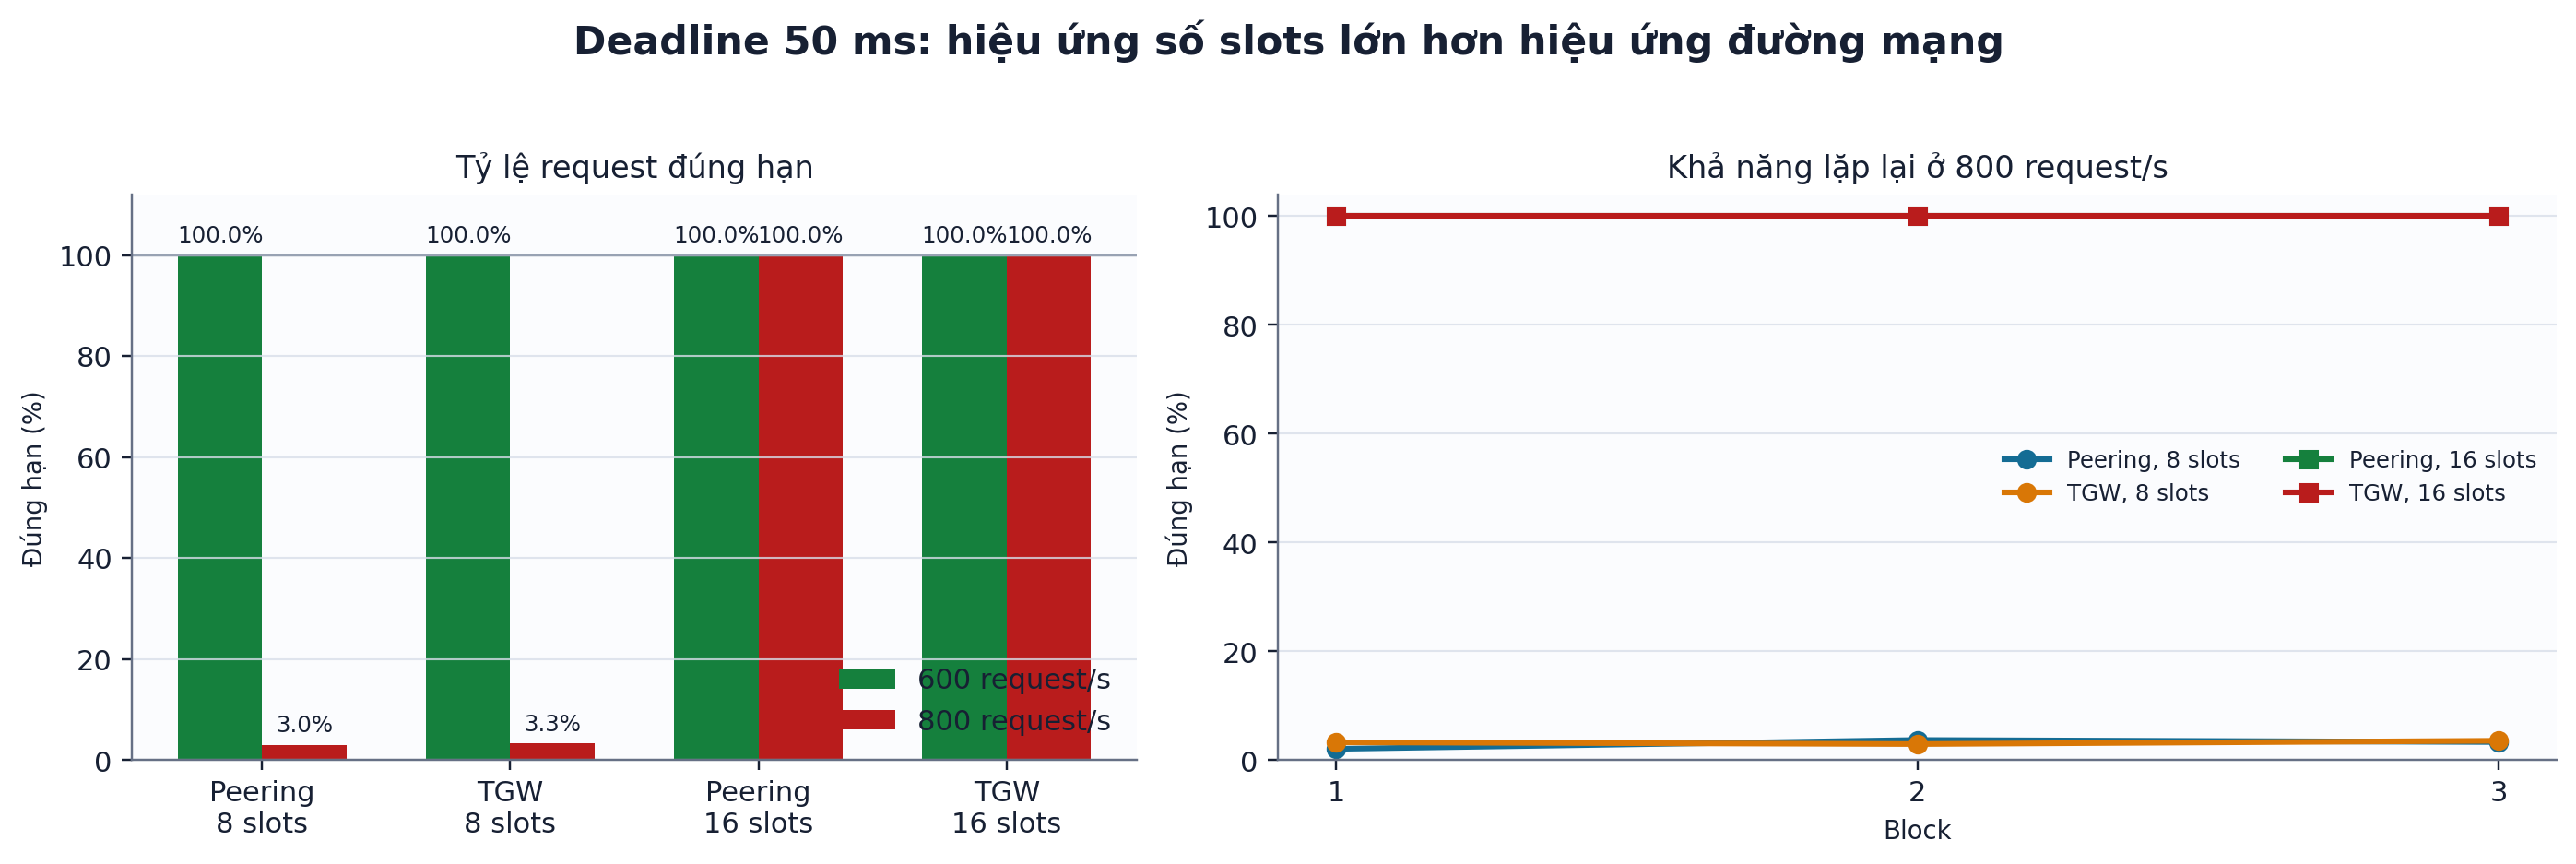
\includegraphics[width=\textwidth]{img/chapter3/primary/application-deadline.png}
\caption{Tỷ lệ đúng hạn và mức lặp lại của hiệu ứng slots trong ba block mới}
\label{fig:deadline-primary}
\end{figure}

Ở 600 request/s, cả tám cấu hình theo mode và slots đều đạt 100\% đúng hạn
trong dữ liệu quan sát. Ở 800 request/s, 8 slots chỉ đạt 1.096/36.000 request
đúng hạn qua Peering và 1.178/36.000 qua TGW, lần lượt 3,0444\% và 3,2722\%.
Khi tăng lên 16 slots, cả hai mode đạt 36.000/36.000 request đúng hạn.

Hiệu ứng $16-8$ slots tại 800 request/s, trung bình qua hai route và ba block,
là 96,8417 điểm phần trăm; từng block nằm trong khoảng
96,5458--97,3167 điểm phần trăm. Vì Peering và TGW đều thất bại với 8 slots và
đều phục hồi với 16 slots, đổi route không giải quyết được giới hạn phục vụ của
worker trong workload này.

\subsection{Cơ chế: tail latency đến từ hàng đợi}

\begin{figure}[H]
\centering
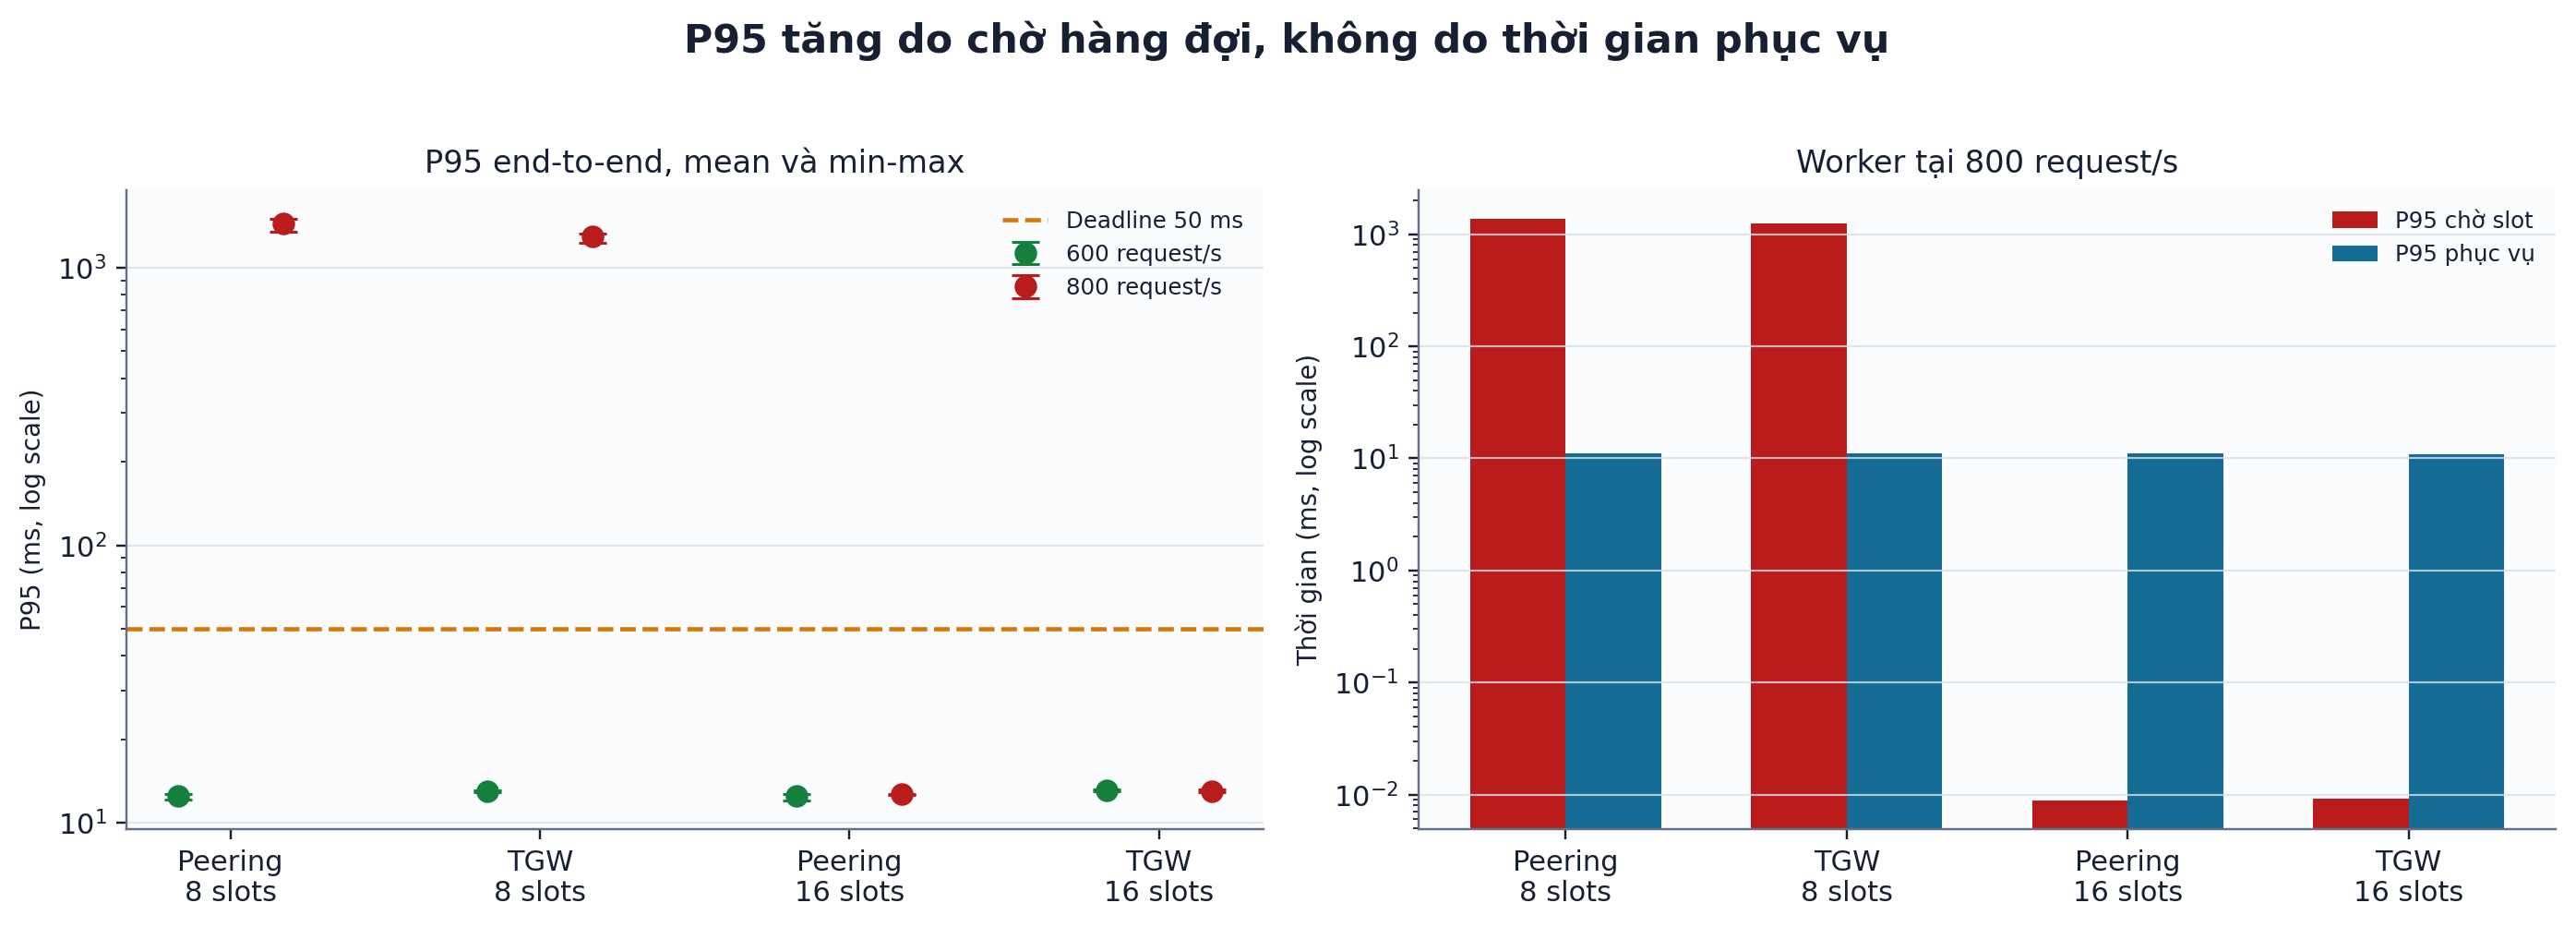
\includegraphics[width=\textwidth]{img/chapter3/primary/application-latency-queue.png}
\caption{P95 end-to-end và phân rã P95 chờ/phục vụ tại worker}
\label{fig:latency-queue-primary}
\end{figure}

Với 800 request/s và 8 slots, P95 end-to-end nằm trong khoảng
1.225,784--1.499,226 ms, vượt xa deadline 50 ms. P95 chờ slot vào khoảng
1,2--1,4 s, trong khi P95 phục vụ vẫn chỉ khoảng 11 ms. Với 16 slots, P95 chờ
giảm xuống dưới 0,013 ms và P95 end-to-end trở lại khoảng 12,651--13,248 ms.
Hình \ref{fig:latency-queue-primary} vì vậy cung cấp chuỗi bằng chứng nhất quán:
tỷ lệ đúng hạn tăng, tail latency giảm, thời gian chờ biến mất, còn thời gian
phục vụ gần như giữ nguyên.

Ví dụ block 3, worker C, Peering, 800 request/s: với 8 slots,
$\lambda_C=732{,}2866$ lời gọi/s và $\overline W_q=0{,}7009511$ s. Định luật
Little trên cohort log hữu hạn cho

\begin{equation}
\overline L_q=\lambda_C\overline W_q
=732{,}2866\times0{,}7009511\approx513{,}2971.
\end{equation}

Với 16 slots ở cùng block/mode/worker, $\lambda_C=799{,}5313$ lời gọi/s,
$\overline W_q=0{,}000005239$ s và $\overline L_q\approx0{,}004189$. Hai giá
trị cho thấy backlog hàng trăm lời gọi đã chuyển thành hàng đợi gần như trống.
Phép tính dùng cùng cửa sổ log và được kiểm tra bằng diện tích occupancy; không
giả định arrival Poisson hay thời gian phục vụ exponential.

\subsection{OpenTelemetry và Grafana}

\begin{figure}[H]
\centering
\begin{subfigure}{0.49\textwidth}
  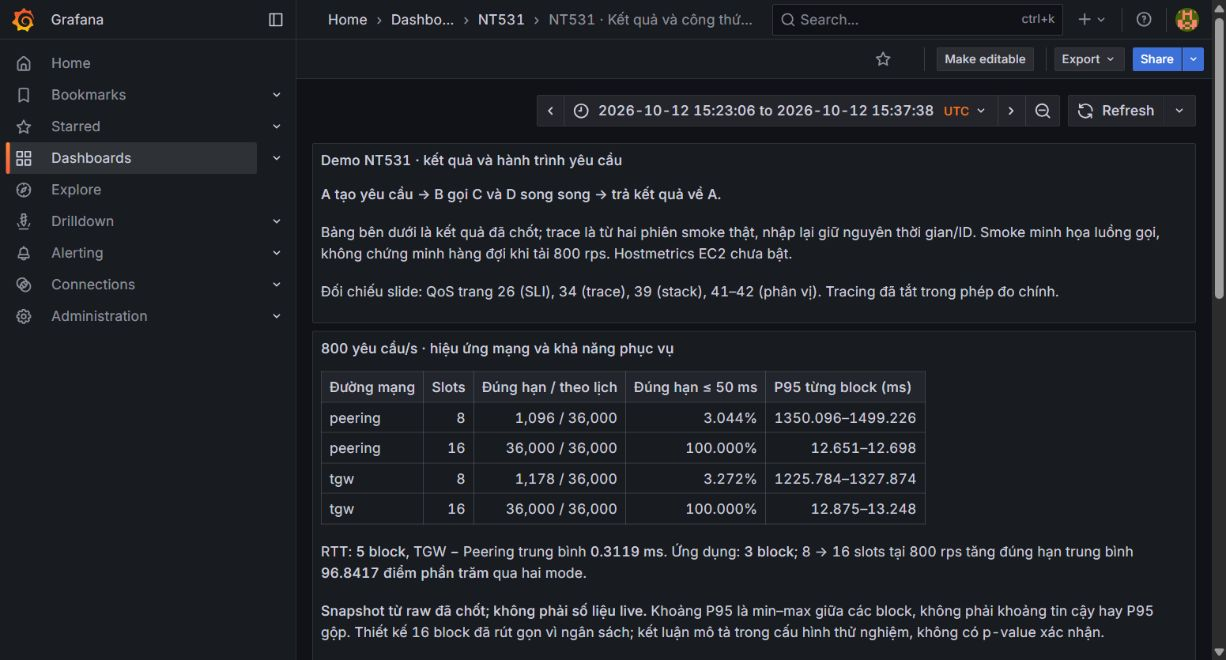
\includegraphics[width=\textwidth]{img/chapter3/observability/grafana-dashboard.jpg}
  \caption{Dashboard tổng hợp}
\end{subfigure}
\hfill
\begin{subfigure}{0.49\textwidth}
  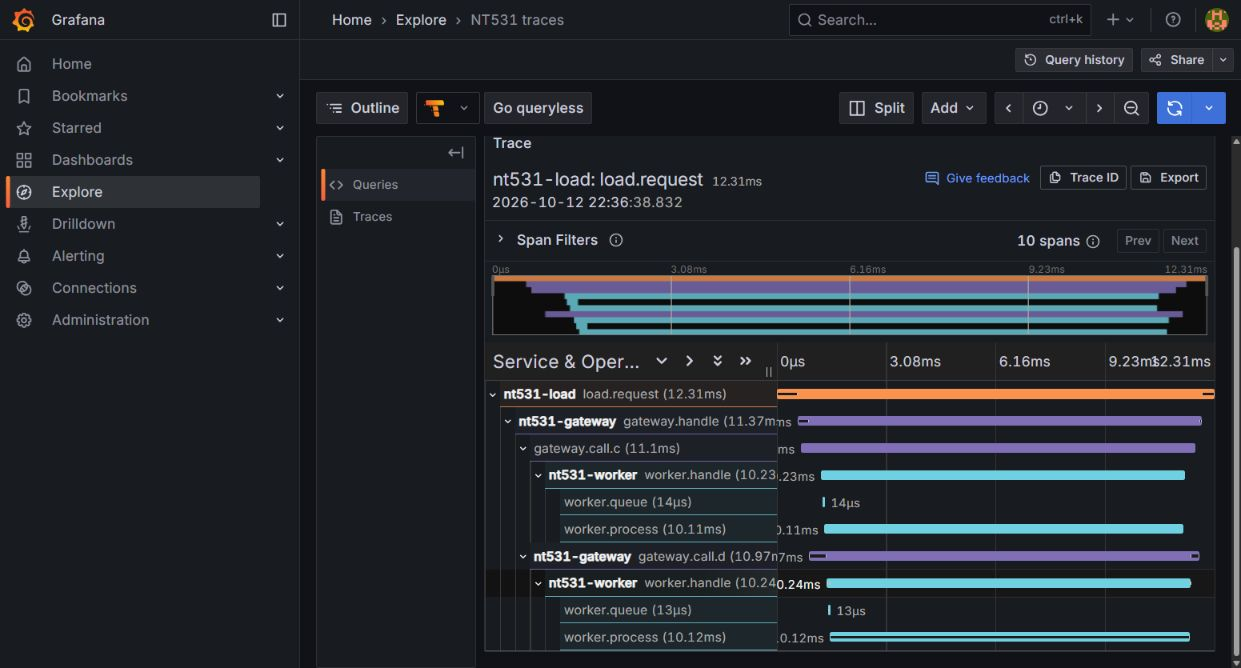
\includegraphics[width=\textwidth]{img/chapter3/observability/trace-waterfall.jpg}
  \caption{Waterfall A--B--C/D}
\end{subfigure}
\caption{Pipeline OpenTelemetry Collector--Tempo--Grafana dùng để giải thích request path}
\label{fig:observability-combined}
\end{figure}

Pipeline đã replay và kiểm tra 12 trace thật, tổng 120 span. Waterfall cho thấy
B gọi C/D song song và cho phép phân biệt queue với service. Trace này là smoke
lịch sử để minh họa cấu trúc request, không phải mẫu benchmark 800 request/s và
không được dùng để tính P95 chính.

\section{Kết luận trực tiếp từ dữ liệu mới}

Ba kết quả mới có mức bằng chứng khác nhau nhưng cùng trả lời một câu hỏi rõ:

\begin{enumerate}
  \item Trong 5/5 block cùng cohort, TGW tăng RTT so với Peering; hiệu ứng ghép
        cặp trung bình là 0,3119 ms.
  \item Tại 800 request/s, đổi Peering/TGW không cứu được cấu hình 8 slots;
        tăng lên 16 slots cải thiện đúng hạn trung bình 96,8417 điểm phần trăm.
  \item P95 phục vụ giữ quanh 11 ms trong khi P95 chờ thay đổi hơn năm bậc độ
        lớn. Hàng đợi ứng dụng là cơ chế chính tạo tail latency trong workload
        này.
\end{enumerate}

Đây là đóng góp mới của đồ án. Kết quả không tuyên bố Peering hoặc TGW thắng
mọi workload; nó chỉ ra khi nào chênh lệch đường mạng đáng chú ý và khi nào
nút thắt ứng dụng lớn đến mức lựa chọn route không còn quyết định SLI.

\section{TCP baseline bổ trợ}

Các phép đo TCP trước đợt xác nhận được giữ làm baseline mạng. Chúng không được
trộn vào năm block RTT hoặc ba block ứng dụng mới vì khác thời điểm và thiết kế.

\begin{table}[H]
\centering
\caption{Tóm tắt TCP baseline lịch sử}
\label{tab:tcp-baseline-summary}
\small
\begin{tabularx}{\textwidth}{>{\raggedright\arraybackslash}p{0.28\textwidth}p{0.17\textwidth}p{0.17\textwidth}X}
\toprule
\textbf{Metric} & \textbf{Peering} & \textbf{TGW} & \textbf{Diễn giải} \\
\midrule
Single-flow receiver goodput & 4,782804 Gbps & 4,608265 Gbps & Peering cao hơn 3,7875\% \\
Fan-in tổng xấp xỉ & 11,611009 Gbps & 11,590520 Gbps & Chênh 0,17646\% \\
CPU busy receiver B & 59,1802\% & 56,8751\% & Không loại trừ bottleneck một core/ENA \\
Jain index fan-in & 0,999133 & 0,984494 & Mô tả chia sẻ trong phiên \\
\bottomrule
\end{tabularx}
\end{table}

Single-flow cho thấy Peering có receiver goodput cao hơn trong hai phiên đã
đo. Tuy nhiên retransmission khác mạnh giữa hai phiên: Peering ghi
48.253--57.185, TGW ghi 0--671. Vì vậy không quy toàn bộ chênh lệch goodput cho
network service.

Trong fan-in, tổng goodput của hai mode gần nhau nhưng receiver B đồng thời ghi
delta lớn ở \nolinkurl{bw_in_allowance_exceeded} và
\nolinkurl{pps_allowance_exceeded}. Ba sender cùng hội tụ vào B nên endpoint
allowance có thể che khác biệt của network path. Kết quả fan-in không phải
equivalence test và không chứng minh hai dịch vụ có throughput bằng nhau.

Baseline TCP trả lời khía cạnh throughput; đợt mới trả lời khả năng lặp lại của
RTT và cơ chế tail latency ứng dụng. Hai lớp bằng chứng bổ sung cho nhau, không
được dùng thay thế lẫn nhau.


\section{Khả năng tái tạo}

Terraform mô tả topology; shell script mô tả workload; raw artifact giữ đầu
vào; JSON phân tích giữ số đầy đủ và SHA256. Báo cáo này dùng số đã được tính
lại từ nguồn thay vì nhập tay từ biểu đồ. Tuy vậy, tái tạo cùng code không bảo
đảm số đo giống hệt vì nền tảng cloud có biến thiên theo thời gian và host.

\section{Nguy cơ ảnh hưởng tính hợp lệ}

Thiết kế hiện tại có năm lượt cho mỗi bộ chính; Peering và TGW được chạy nối
tiếp, chưa counterbalance đầy đủ. Bandwidth burst, placement và nhiễu nền của
EC2 không được kiểm soát trực tiếp. Trong fan-in, ba wrapper không bắt đầu tuyệt
đối đồng thời và ENA tại B được chụp cho cả phiên. Receiver B có thể trở thành
bottleneck dùng chung. Các điểm này giới hạn causal attribution: kết quả là
end-to-end observation của cấu hình đã đo, không phải service limit riêng của
Peering hoặc TGW.
